\chapter[Diagramme structure -- temps: remprésentation graphiques de la
dynamique d'une population structurée][Diagramme structure -- temps]{Diagramme structure -- temps: remprésentation graphiques de la
dynamique d'une population structurée}\label{Chap:STDiag}

\vspace{4cm}

\begin{Spacing}{1}
\texttt{
Le Bourlot, Vincent, François Mallard, Caroline Ligier, Manuel Massot, 
David Claessen, and Thomas Tully, "A simple graphical method for 
displaying structured population dynamics and STdiag, its implementation 
in a R package".\\
under review at Journal of Animal Ecology
}
\end{Spacing}

\section*{Abstract}
\addcontentsline{toc}{section}{Abstract}

%\begin{enumerate}
  %\item 
  
  \lettrine[lines=3]{I}{n demography}, a detailed study of the temporal dynamics
  of a population structure is often required to better understand the processes that
  underline the overall dynamics and the individual life histories.
  %\item 
  
  Heatmaps using time and structure (such as size-structure) as x and y
  coordinates and density as colors are efficient tools for displaying the
  dynamics of a structured population. Such representations (structure--time
  diagrams), reveal the data at several levels, from general outlook to fine
  details.
  %\item 
  
  This graphical display is a simple and efficient way to make large
  demographic datasets coherent and to disclose the underlying often hidden
  demographical processes. But despite its efficiency, this method has been
  scarcely used in ecology and demography.
  %\item 
  
  To emphasise how rich this graphical representation is and to illustrate
  that this method can be applied even outside the field of ecology, we present
  three case studies:  a long-term survey of a collembolan population in a
  laboratory microcosm, a 16 years old survey of wild common lizard population and
  the antibiotics consumption in France during one year.
  %\item 
  
  We present the R package STdiag, an interface to complex graphical
  functions to easily produce such "structure--time diagrams" from raw datasets.
  This package available for all operating systems via R-Forge. Its syntax and
  options are described, discussed and illustrated using our three examples.
%\end{enumerate}

\section{Introduction}

Structured populations are complex assemblages of individuals differing in age,
reproductive stage or physiological state such as size or body condition (Figure
\ref{Fig22-1}a, b). Different approaches have been used to display structured
population dynamics (Figure \ref{Fig22-1}c, d, e): By displaying the whole population size fluctuations,
the structure is not taken into account (Figure \ref{Fig22-1}c) \autocites{schrautzer2011a}.
The structure can be roughly considered by splitting individuals into separate
groups (of size or stages) whose dynamics can be displayed on adjacent plots
\autocites{plaistow2009a} or, to facilitate comparisons, on overlaid curves (Figure
\ref{Fig22-1}d) or on a stacked bar plot (Figure \ref{Fig22-1}e) \autocites{madsen2000a}. But condensed
three-dimensional diagrams are required to finely display the structure dynamic
especially when the structuring factor is continuous (size, age). These diagrams
encompass “event history diagrams” that allow the graphical representation of
life history traits at the individual level of a whole
cohort\autocites{carey1998a,carey2008a} or the production of “shaded contour
maps” such as the ones used to represent the temporal dynamics of
aged-structured demographic rates such as death or birth rates in human
populations \autocites{vaupel1997a,vaupel1998a}.These graphical representations
are mainly used in human demography to represent secular changes in
age-dependent demographicrates
\autocites{vaupel1987a,vaupel1997a,vaupel1998a,andreev2000a,erlangsen2003a}.
To our knowledge, despite their interest, such powerful visual displays have
almost never been used in ecology to represent the temporal dynamics of
structured populations \autocites{faerovig2002a}. This may result from the
prohibiting cost of publishing colours pictures. But with the development of
online publishing, colour methods are becoming more widely used.
The R software \autocites{team2012a} is a language and environment for data
manipulation, calculation, statistical computing and graphic display. R provides
libraries such as \texttt{lattice} \autocites{sarkar2008a} or \texttt{ggplot2}
\autocites{wickham2009a} to produce heatmaps.
But although higly customizable, the plotting functions are often difficult to
handle for beginners.

\begin{figure}[!ht] % Figure 1 
\centering
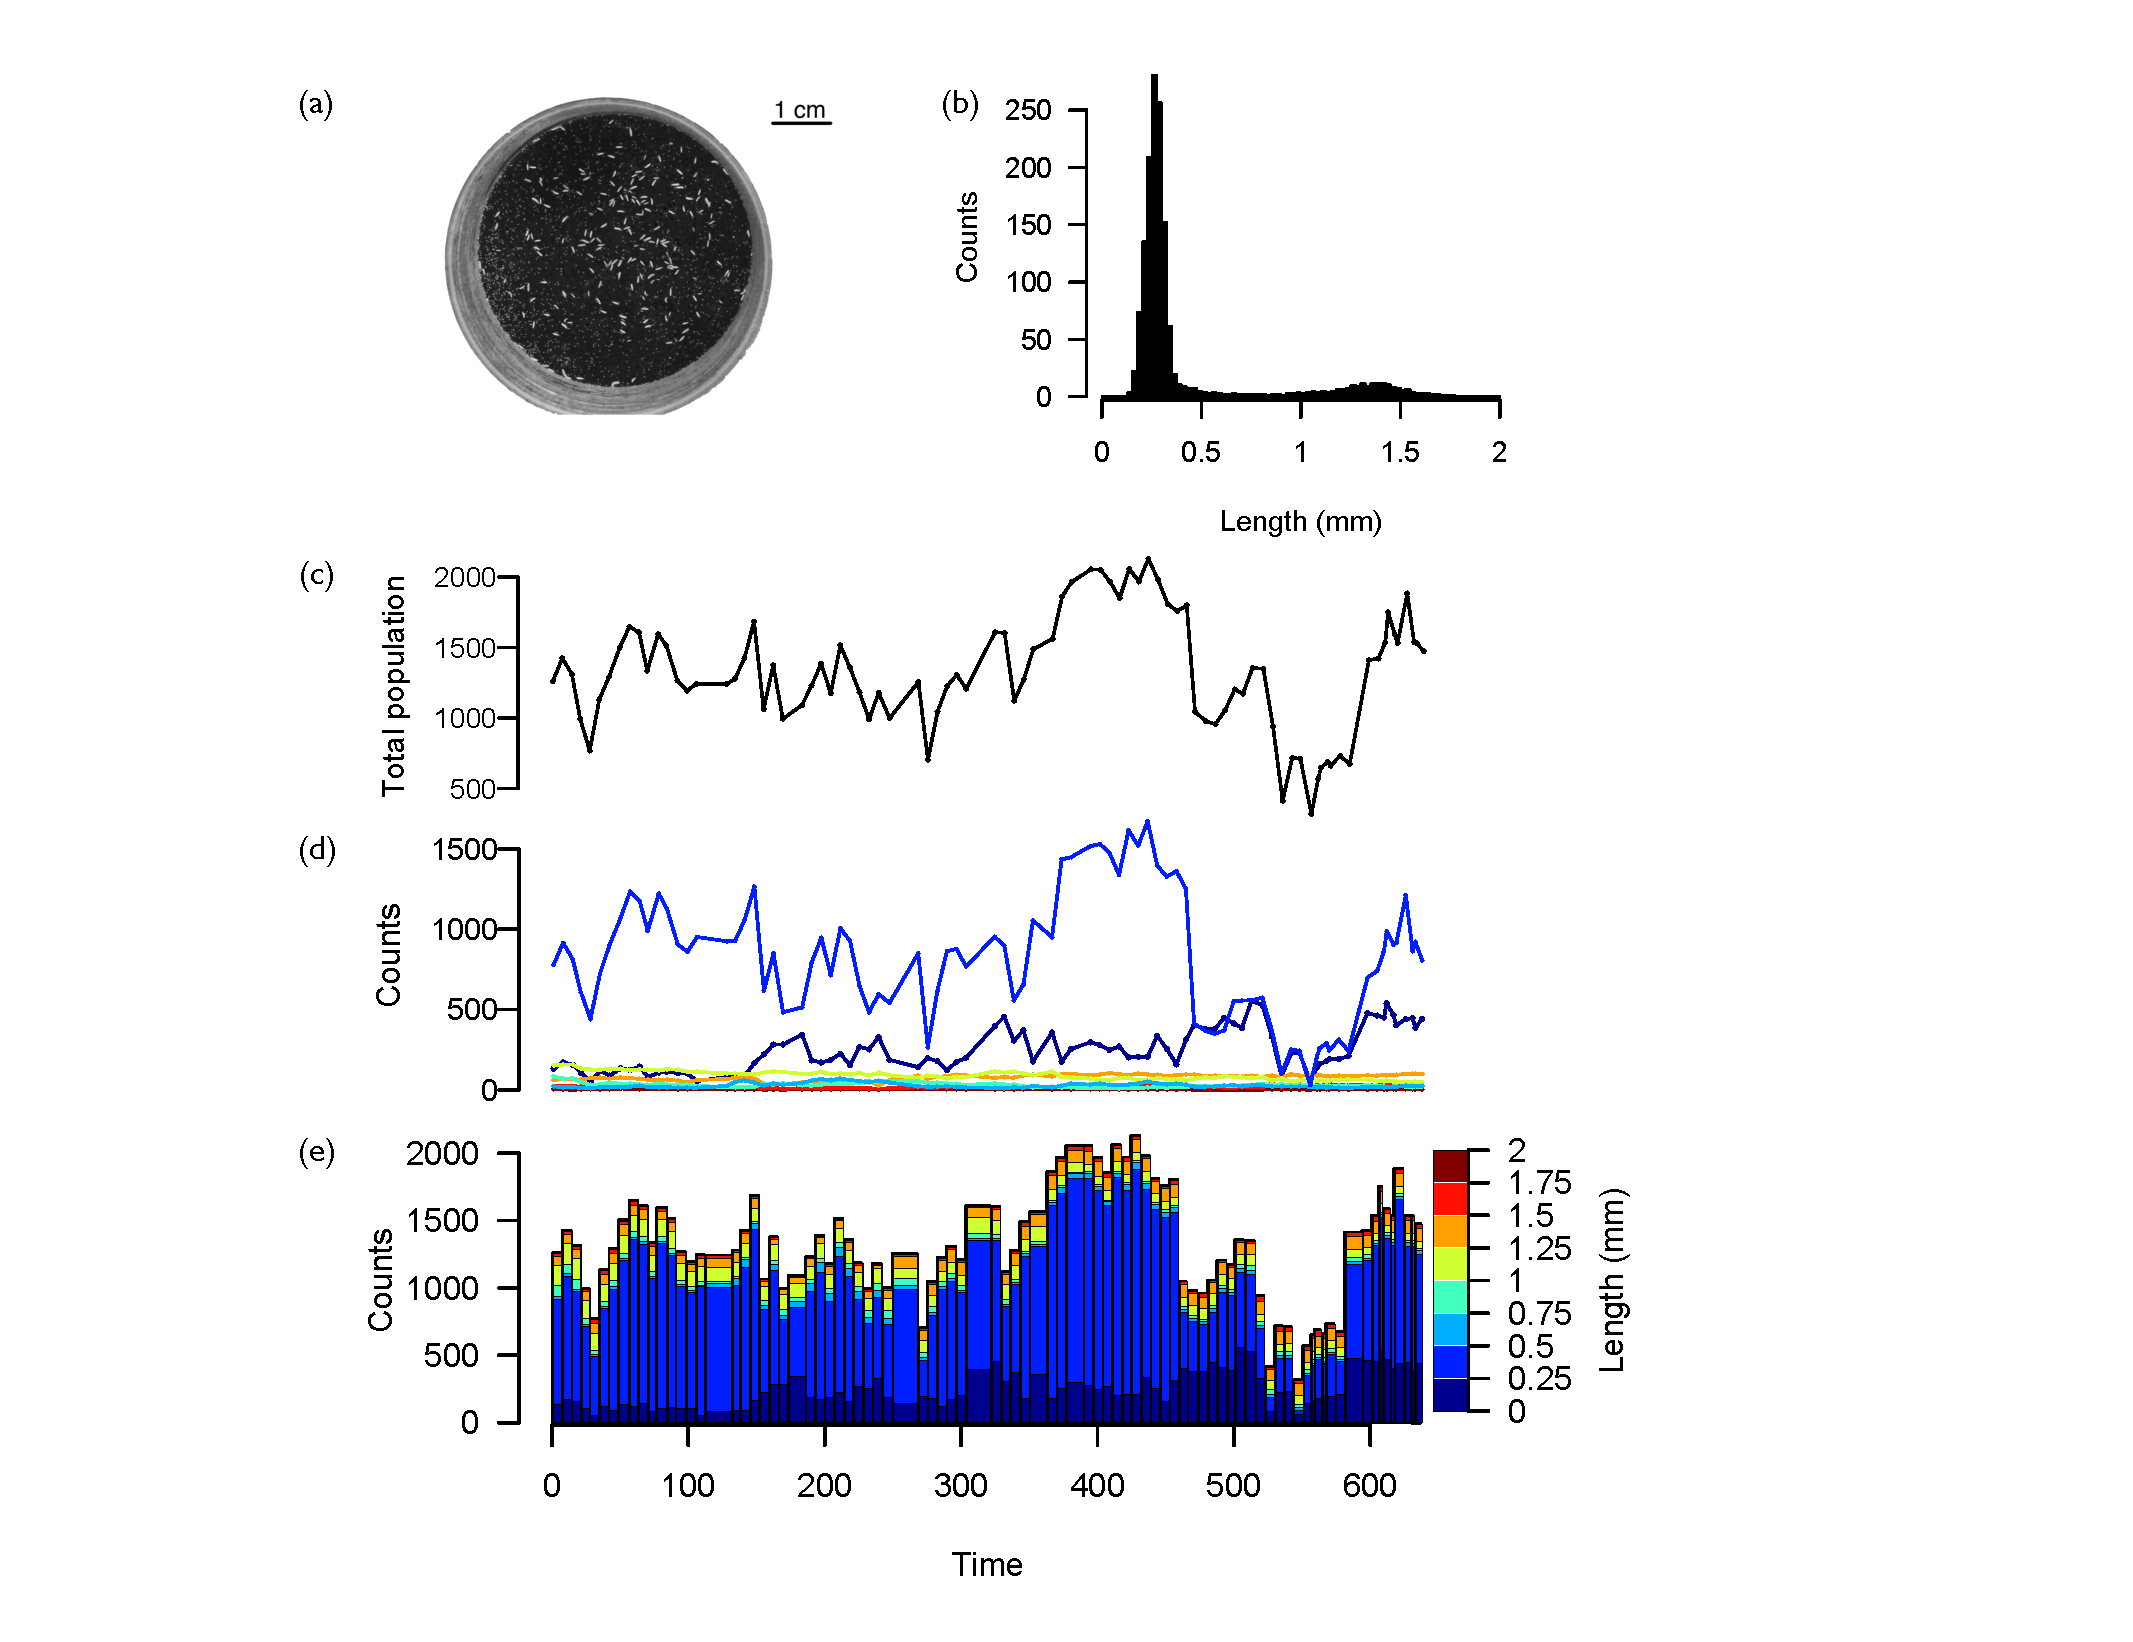
\includegraphics[height=0.75\textheight]{2_Methodo/Fig/Fig22-1.pdf}
\caption[\lofimage{2_Methodo/Fig/Fig22-1.pdf}Classical representation of a
population structure]{ We used as a practical example an experimental population
of the Collembola \textit{Folsomia candida} (a) whose structure has been measured every one or two weeks . The size structure at one time is classically shown as a histogram (b) and the total population dynamics on a time series plot (c). To represent both the structure and temporal dynamics, the population has been divided in
several size classes to plot their dynamics independently (d) or to produce a
stacked bar plot (e). While these representations underline the dynamics inside
each size classes, the patterns of dynamics between adjacent classes remain
hidden.great confidence.
}
\label{Fig22-1}
\end{figure}


We made the R-package \texttt{STdiag} to provide a user-friendly interface for
representing time series of structured populations using heatmaps. We detail how
to generate such graphics and discuss their biological interests using (1) the
long-term structure dynamics of experimental laboratory populations of the
Collembola \textit{Folsomia candida} (Figure \ref{Fig22-2}), (2) a long term study of a population of
common lizards Zootoca vivipara in France (Figure \ref{Fig22-3}) and (3) an example in the
field of pharmaco-epidemiology: the seasonal dynamics of the annual consumption
of antibiotics in France (Figure \ref{Fig22-4}).

\section{Method overview}

The diagram produced by \texttt{STdiag} shows a structuring element (age, size,...) along
the $Y$-axis and time along the $X$-axis. These variables are usually continuous
but have to be made discrete and then put into several classes, the number and width
of which depend on the quality and size of the available dataset. For each time
and structure class coordinate, a colour rectangle is plotted whose hue refers
to the number of individuals (or any other statistics such as frequency or rate)
in that class (possibly on a logarithmic scale) at the given time. This
representation puts side-by-side colour histograms for each time value and
emphasises the temporal dynamics according to the structure of the population.

\section{Package STdiag usage}

To easily display the dynamics of a structured population we made the package
\texttt{STdiag} which is freely available at R-forge (\url{R-forge.r-project.org/}) and
can be installed in R with the following command:

\begin{verbatim}
install.packages('STdiag',repos="http://r-forge.r-project.org")
\end{verbatim}

\subsection{Importaing and formating the data}

\subsubsection{Data frame.}
\texttt{STdiag} uses the lattice function \texttt{levelplot}
\autocites{sarkar2008a}.
As a consequence, the basic data format is a three column data frame containing the
$X$ (time), $Y$ (structure such as age or size) and $Z$ (number of individuals)
coordinates. The data frame has $TxS$ lines where $T$ is the number of time
values and $S$ the number of structure classes.

\subsubsection{Matrix.}
Another possibility is to use a matrix description of the data using two vectors
$x$ and $y$ of size respectively $T$ and $S$ for the time and structure
coordinates, and a matrix $z$ of size $TxS$ containing the number of individuals
at each coordinate. This mimics the format used by function image \autocites{team2012a}.
In case one wishes to use the frame format for data in the matrix format, the
function \texttt{Matrix2DataFrame} is provided:
\begin{verbatim}
DataFrame <- Matrix2DataFrame(z, x, y, xlab="time", ylab="structure",
zlab="number").
\end{verbatim}

\subsubsection{Individual based data.}
The function \texttt{Indiv2DataFrame} is also provided to convert
individually based data to a data-frame that can be plotted with \texttt{STdiag}. This function handles a
data-frame containing one line per individual and, for each individual, the time
of the observation in the first column and the value of the structure in the
second one. The option classes, allows to control the number of classes to
discretize the structure variable. A single value produces the wanted number of
regular classes (default set to $50$), whereas a vector specifies the breaks of
the classes as in function hist. This function is used as follows:
\begin{verbatim}
DataFrame <- Indiv2DataFrame(IndivData, classes=50).
\end{verbatim}

\subsection{Generating the plots}

\subsubsection{Data frame.}
The simplest way to generate the basic plot is to use the data frame
formulation. If the columns of the data frame are in a time-structure-number
order, a simple call to
\begin{verbatim}
STdiag(DataFrame)
\end{verbatim}
will produce the plot. If one wants to specify what column to plot, the function
\texttt{STdiag} accepts the formula syntax:
\begin{verbatim}
STdiag(number ~ time * structure, data= DataFrame).
\end{verbatim}
In any of those or the following forms, the vector used as time can either be a
numeric vector or a vector of dates of classes \texttt{POSIXlt},
\texttt{POSIXct} or \texttt{Date}. Class \texttt{factor} is not yet supported
for date format.

\subsubsection{Matrix.}
To use the matrix formulation, call either
\begin{verbatim}
STdiag(Matrix)
\end{verbatim}
in which case $X$ and $Y$-axes will be default vectors from $1$ to respectively
$T$ and $S$. Or, if one wants to specify the $x$ and $y$ coordinates,
\begin{verbatim}
STdiag(x=time, y=structure, z=Matrix).
\end{verbatim}

\subsection{Improving the graphical representation}

Our method is implemented with several options to adjust the plot to be as
informative as possible.

\begin{figure}[!ht] % Figure 2 
\centering
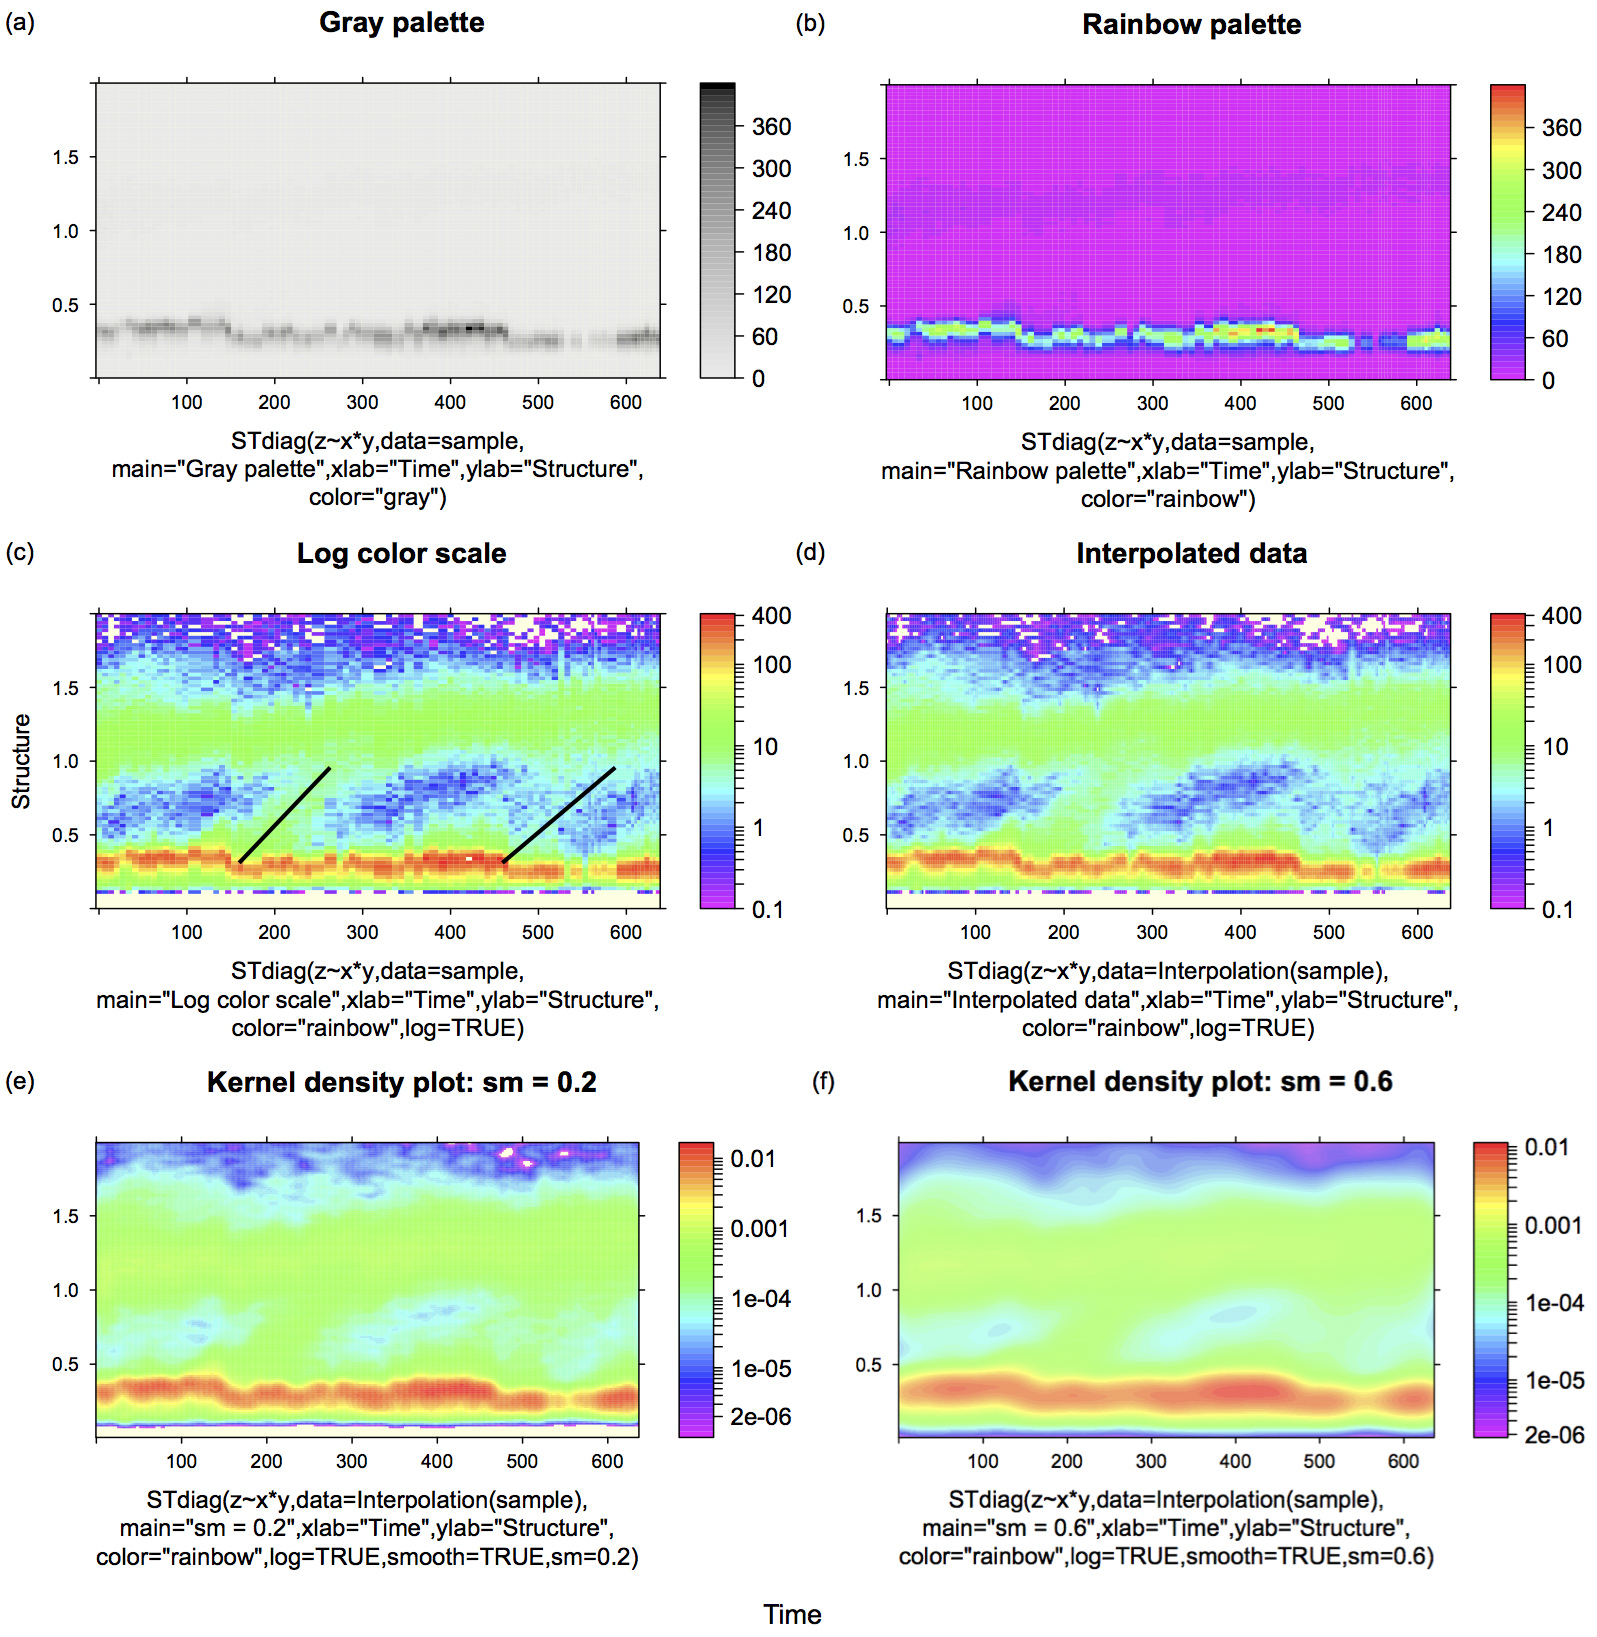
\includegraphics[height=0.70\textheight]{2_Methodo/Fig/Fig22-2}
\caption[\lofimage{2_Methodo/Fig/Fig22-2}Collembolan population dynamics plotted
with STdiag]{ Collembolan population dynamics plotted with STdiag. The code to produce each plot is given in each panel. Length is discretised into classes of
0.05mm length. Number of individual at each date length coordinate is
represented on a linear grey (a) or colour (b) scale or on a logarithmic scale
(c, d). Panel (d) represents an interpolated version of panel (c). Panels (e)
and (f) represent two kernel density estimates with increasing smoothness. The
population is mostly composed of small individuals ($\approx0.4$ mm) living with some
adults ($\approx1.2$ mm). Logarithmic scale reveals details about the recruitment of
some cohorts, the growth rate of which can be estimated (black lines, c).
}
\label{Fig22-2}
\end{figure}

\subsubsection{Colour palette.}
The readability of the diagram partly relies on the choice of colours for the
palette (Figure \ref{Fig22-2}a, b). The hues are sorted following either a gray scale from
pale gray to black or a rainbow gradient (Figure \ref{Fig22-2}a, b, c).This can be adjusted
using the option color="palette" inside \texttt{STdiag()} where palette can be
one of the following: \texttt{gray, topo, terrain, heat, cm, rainbow} or by
default \texttt{tim} (see tim.colors in library fields, \citealp{furrer2012a}).

\subsubsection{Logarithmic scale.}
When the number of individuals in the different classes differs by several
orders of magnitude (Figure \ref{Fig22-1}b) we recommend using a logarithmic scale to increase
the readability of the generated graphics. The option
\texttt{log=TRUE}$/$\texttt{FALSE} allows the user to switch easily between
linear and logarithmic colour scales.

\subsubsection{Interpolation.}
The quality of the diagram can sometimes be improved by applying an
interpolation to smooth the representation and link together uneven time
intervals by creating evenly spaced data (Figure \ref{Fig22-2}d).The interpolation method
create an artificial dataset with evenly distributed data, based on the original
data. It is essential to make a clear distinction when reading such a diagram
between the real data and data created by the interpolation and we recommend to
first use a non-interpolated representation of the data. To interpolate the
data, we provide in the package the function Interpolation. This function is an
interface to function interp.surface in package fields adapted to quickly handle
data accepted by function \texttt{STdiag}. It takes as argument the data frame
to be interpolated in the form of three columns: time, structure and number of
individuals, in that order. The options \texttt{intervX} and \texttt{intervY} allow the user to
manually choose the intervals between two interpolated points, respectively over
$X$ (time) and $Y$ (structure) axes. If those options are left empty, the
function uses the minimum distance between two points in the first and second columns as
intervals for respectively $X$ and $Y$ axes.

\subsubsection{Kernel density estimate.}
The function STdiag~provides an option \texttt{smooth=TRUE}$/$\texttt{FALSE} to
plot a weighted kernel density estimate of the data using an axis-aligned bivariate normal
kernel, where the data are the time-structure coordinates weighted by the number
of individuals. The estimate is derived from the function \texttt{kde2d} in
package \texttt{MASS} \autocites{venables2002a}. The density estimate can be
adjusted with options sm, a positive scalar ($0$ meaning the original data and $1$ being
the normal reference distribution kernel estimation bandwidth) defining the smoothness of
the kernel density estimate, and $n$, the number of points on the $X$ $Y$ grid.
Together, these options allow to view a smooth representation of the structured
data (Figure \ref{Fig22-2}e, f, Figure \ref{Fig22-3}). Contrary to the interpoation, the kernel density
estimate only provides a smooth representation of the data. In the case of
missing data, such as irregular time intervals, interpolating the data before
plotting the kernel density can avoid having gaps in the density for a low
smoothing factor (small \texttt{sm}).

\section{Reading and interpreting ST diagrams}

\subsection{Dynamics of a laboratory population of collembolan.}
We used as a first practical example of temporal dynamic of a structured
population, some data issued from the close follow-up of an experimental
population of a springtails maintained in our lab during about $600$ days. We
studied the species \textit{Folsomia candida} that is commonly used in laboratory and is
easy to breed and maintained \autocites{fountain2005a}. This is
an ametabolous parthenogenetic hexapod whose populations are composed only of females of
different size because the juveniles look like minute adults and the adults
continue to mould and grow after reaching maturity. The individuals were bred at
$21 \degres$C in cylindric plastic boxes of $5.3$ cm diameter with a $3$ cm thick
plaster substrate to keep the environment damp \autocites{tully2008a} (Figure
\ref{Fig22-1}a). The population is fed weekly with a mix of yeast in agar-agar in a fixed quantity
and kept in the dark the whole time. Measures of the number and size of
individuals are taken every one or two weeks using picture analysis with the
image processor ImageJ \autocites{abramoff2004a,mallard2012a,mallard2013a}
providing the structure of the population at each time of measure (Figure \ref{Fig22-1}b).

The structured time diagram (Figure \ref{Fig22-2}) immediately reveals the predominance of the
younger class ($<.5$ mm). The use of a log scale (Figure \ref{Fig22-2}c),
reveals some inter-class dynamics undetectable using classical representations: between day
$150$ and day $300$ a cohort of small individuals grows and recruits into the
adults. This visual display allows one to estimate some demographic parameters
that cannot be read on classical representations (Figure \ref{Fig22-1}): size at
birth ($\approx0.28$ mm, by observing spikes of births), adult length ($1.9$ mm around
day $50$), growth rate of a cohort of juveniles fighting to be recruited in the
population ($0.22$ mm.month$^{-1}$, slope of the straight line of Figure
\ref{Fig22-2}c).

\subsection{Dynamics of a wild population of common lizards.}

As a second study example we used individual-based mark-recapture data collected
from 1989 to 2004 in a population of common lizards from the Mont Lozère in
southern France ($1420$ m a.s.l, $44\degres30$’N, $3\degres45$’E). Data collection
each year was structured as follows: a capture session of yearlings ($1$ year
old individuals) and adults in June-July and a temporary transfer of pregnant females to the
laboratory to mark and measure juveniles from birth \autocites{le-galliard2010a}.
The Figure \ref{Fig22-3} reports the size structure (snout-vent length) of the
population. We used a total of $7486$ measurements, $3935$ females and $3551$
males.

The Figure \ref{Fig22-3} clearly shows the long term dynamic of the population structure:
males are on average smaller and less captured than females. Compared to other
exemples, the dynamic of the population structure is relatively discontinuous
(Figure \ref{Fig22-3}). The population structure is multimodal along the size axis because of
the annual reproduction, and is discontinuous along the time axis because the
sampling was not perfomed during the six months of the hibernation period. The
sampled population is composed of newborns ($\approx2$ cm), yearlings ($\approx4$ cm) and
adults ($>5$ cm). The figure also shows at a glance some secular changes in the
mean size of both adults and yearlings: the body length in the population increases from
1989 to 1994 \autocites{chamaille-jammes2006a} and decreases
thereafter.

\begin{figure}[!ht] % Figure 3 
\centering
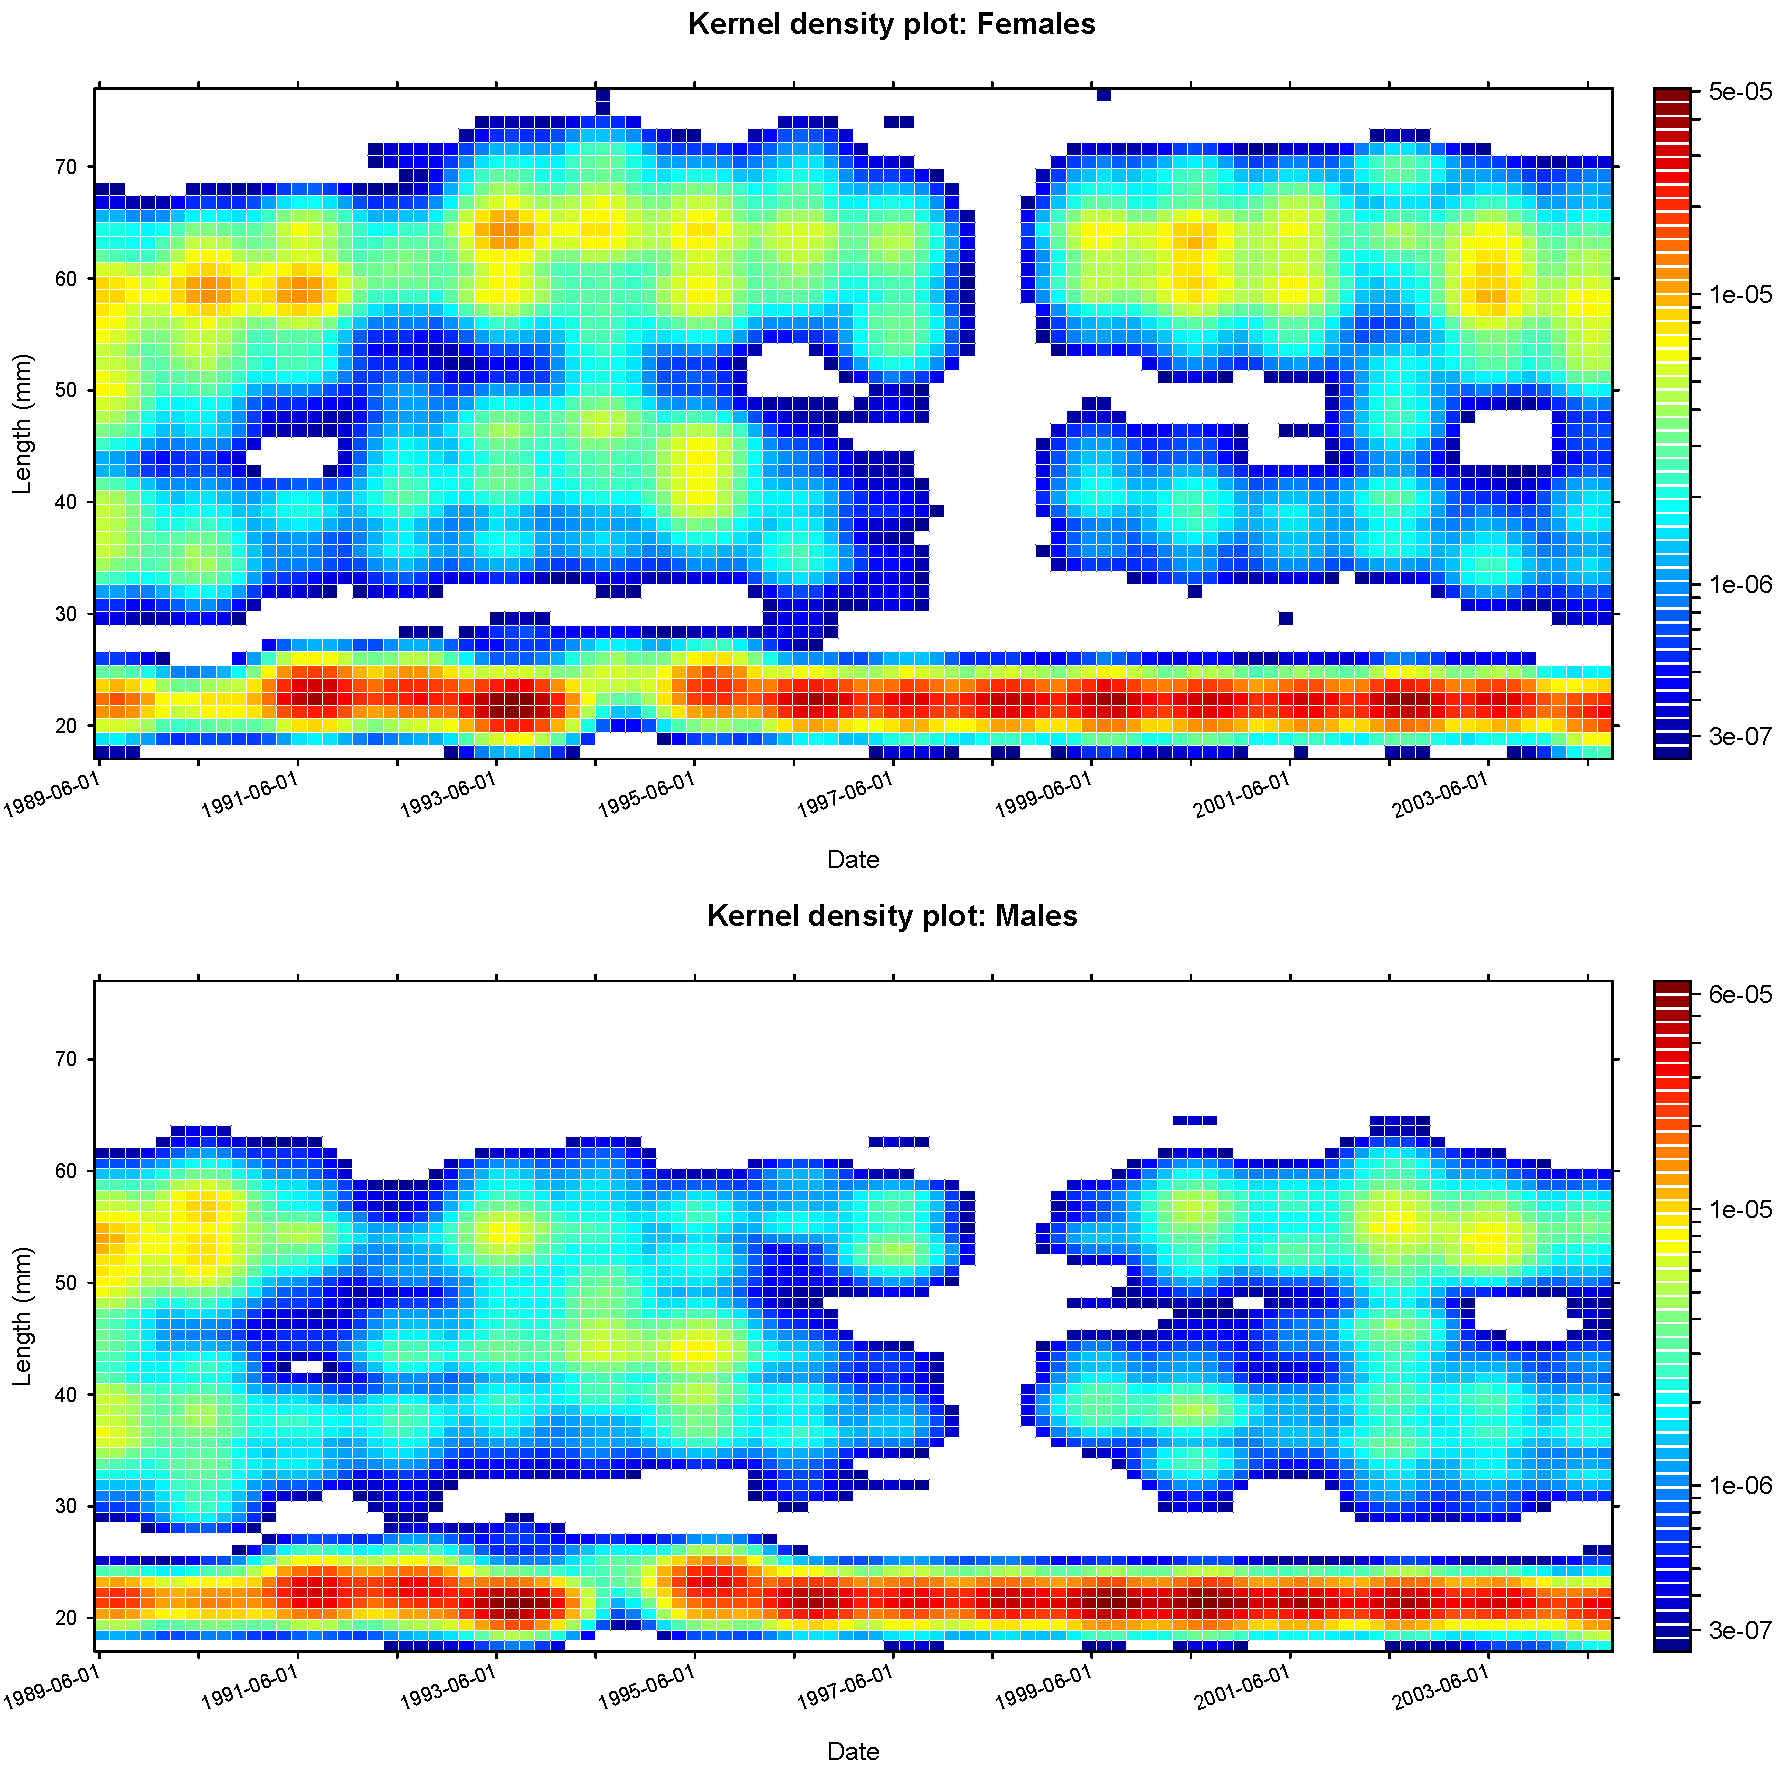
\includegraphics[width=0.85\textwidth]{2_Methodo/Fig/Fig22-3.pdf}
\caption[\lofimage{2_Methodo/Fig/Fig22-3.pdf}The follow-up of a population of the common lizard]{ The follow-up of a population of the common lizard. The plots represent the
population size structure (snout-vent length) of the animals (females, first
row, and males second row) captured in the population each spring. Capture
pregnant females are kept in the laboratory until parturition and the juveniles
are measured right after birth. In 1998, for exceptional reasons the prospection
effort was very low and very few adults of sub-adults have been captured and
measured. The population structure and the long term changes of snout-vent
length can be easily seen on these graphs. We used here a log scale and a kernel
density plot. The large "dots" that are apparent with regular frequency on the
Female plot result from the seasonal annual census of the population.
}
\label{Fig22-3}
\end{figure}


\subsection{Antibiotics consumption}

Our last example -- the consumption of antibiotics in France -- is an
application of our method in the field of pharmaco-epidemiology. It illustrates the
powerfulness of this graphical display to make database of tens of millions of
observations almost instantaneously understandable. We have used data from the
French national database provided by the CNAMTS (“Caisse nationale d’assurance
maladie des travailleurs salariés”, national fund of health insurance for
employees), which covers $75\%$ of the French population. In this specific
example, one can easily see that the purchase of antibiotics decreases every
weekend and during public holiday because most of the chemist shops are closed
(vertical bars on Figure \ref{Fig22-4}a). One can see also that on average, more antibiotics
are purchased for children than for adults. But more interestingly, the plot
reveals the seasonal change in antibiotic consumption for each age class in the
population (Figure \ref{Fig22-4}a):  the seasonal variation in children antibiotic consumption
follows the periods of holidays while for adults and elderly people, the plot
(Figure \ref{Fig22-4}a) specifically underlines the detailed topology of the burden of
purchases that has arisen during the H1N1 influenza pandemic which occurred from
September 2009 to January 2010 in France (Figure \ref{Fig22-4}b, c;
\citealp{lemaitre2010a,lemaitre2012a}).

\begin{figure}[!ht] % Figure 4 
\centering
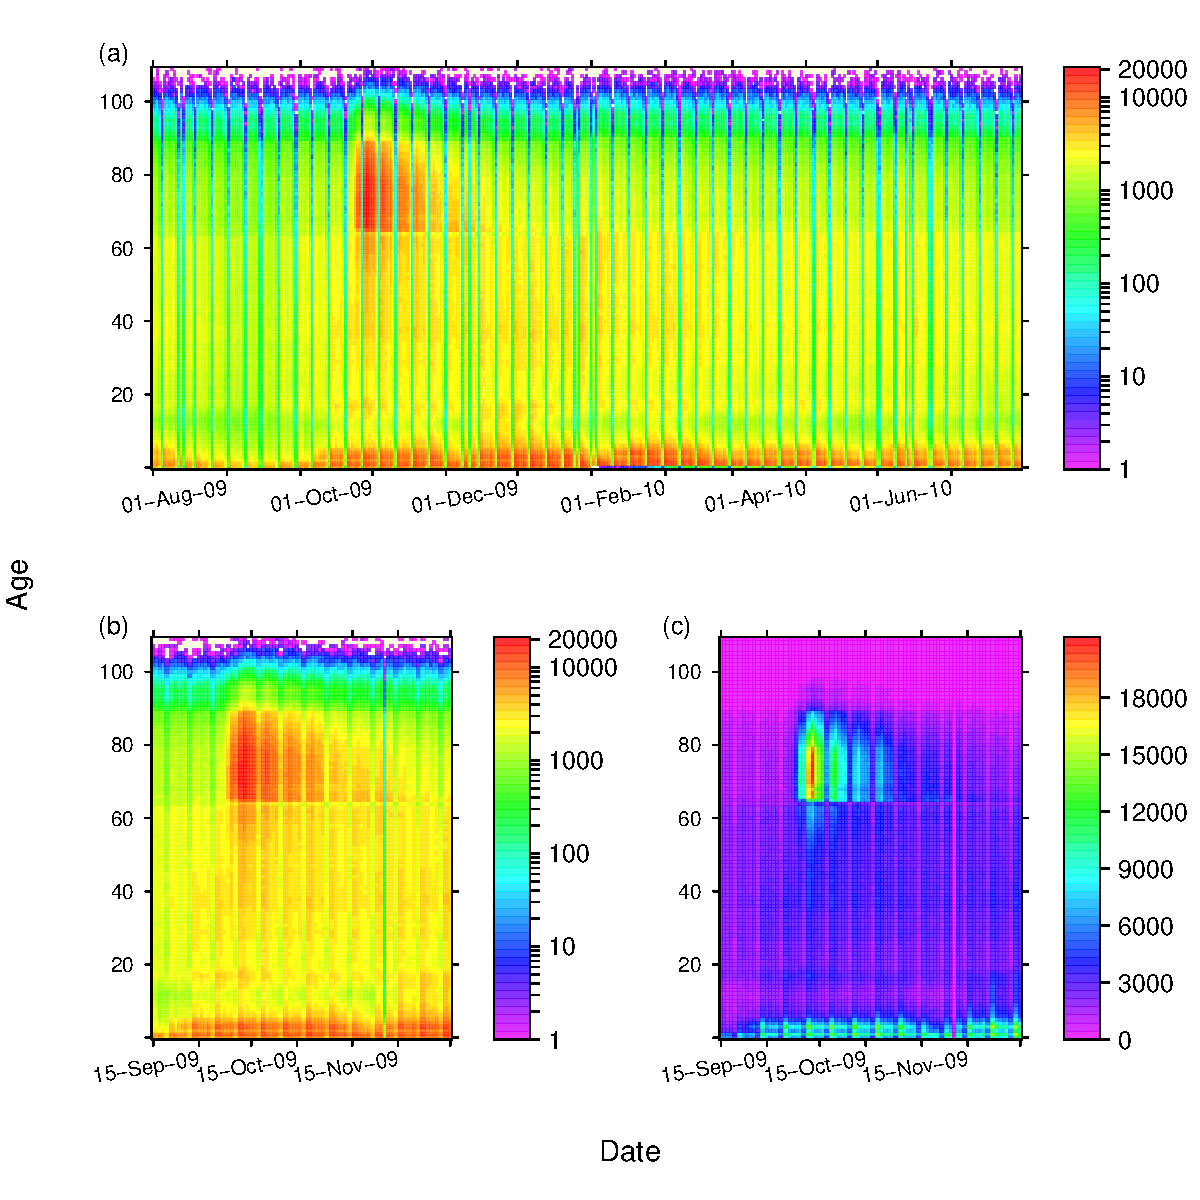
\includegraphics[width=0.85\textwidth]{2_Methodo/Fig/Fig22-4.pdf}
\caption[\lofimage{2_Methodo/Fig/Fig22-4.pdf}Antibiotic consumption in France]{ Graphical representation of the antibiotic consumption in France from 1st July
2009 to 30th June 2010. The number of antibiotics bought in chemist’s shop is
shown for each age class (68 millions of observations). (a) The full
representation reveals the structure by week (the purchases of antibiotic falls
off during the weekend and public holiday), the seasonal fluctuations (less
consumption during spring and summer seasons) and a wave of consumption in
autumn 2009. The vacations give rhythm to the children’s antibiotic consumption.
Removing saturday and sunday allows a cleaner view of the data, and a close-up
view on the autumnal wave of purchases on a logarithmic (b) or linear (c) scale
reveals the increase in antibiotics consumption following the outburst of H1N1
during that period.
}
\label{Fig22-4}
\end{figure}


\section{Conclusion}

A multi-dimensional diagram such as our structure--time diagram (Figure \ref{Fig22-2}b) is
preferred to a simple time series representation (Figure \ref{Fig22-1}c, d) for several
reasons: time series representation lacks the continuity of the structuring
element. Although time series plots and time series analyses are very powerful
and bring useful information on dynamics inside classes that are artificially
created, such as number of individuals or existence or not of a periodicity, the
small number of classes usually used and the representation in lines make it
very difficult to read and therefore detect and analyse any cross classes
dynamics. A three-dimensional diagram offers a unique and complete visual
display of the variations of the population structure and is thus a very
powerful tool for the description of a population and a convenient way of
guiding the analysis. Moreover, by juxtaposing several structure--time diagrams
one can add an extra dimension to the graphical display, such as the sex of the
individuals as in the lizard example (Figure \ref{Fig22-3}) or any other categorical variable
(population, genotype etc.). If one uses the same axis for these diagrams, one
can in a glance compare the complex dynamics of several categories of
individuals.

The structure--time diagram does not need individuals to be identified from one
time to the other. And without any individual trajectories, changes in the
structure over time directly draw dynamics of cohorts (as in Figure \ref{Fig22-2}c).

STdiag can also be used to represent any type of data with a structuring factor
and an aggregate statistic. For instance, this method can be used to represent
the average mortality rate in each age-time class \autocites{vaupel1987a}, or the evolution over time of the average size depending on the age,
illustrating the shrinkage of Soay sheeps \autocites{ozgul2009a}. It
can also be used for displaying data from a population model such as a physiologically
structured one \autocites{metz1986a}. It can also be applied to
follow the temporal dynamic of a human population structure coming for instance from
medical survey to detect any secular or seasonal changes for example (Figure \ref{Fig22-4}).

Such diagrams fulfil the criteria for excellence in statistical graphics
\autocites{tufte1990a}: they show many numbers within a small space (high
data density) thus making coherent large data sets without distorting the data; they reveal the
data at several levels of detail, from fine structure to broad overview,
encourage the eyes to compare different pieces of data and induce the viewer to
think about the substance rather than about the method \autocites{tufte2001a}.

With the development of automatic data acquisition and prolific databases
\autocites{le-galliard2012a,mallard2012a,mallard2013a}, the use of such a
graphical display should become more common in population ecology but also in many other fields such as epidemiology or medical
surveys.

\section{Acknowledgments}

We thank the Programme interdisciplinaire du vivant Longévité et vieillissement
funded by the Centre National de la Recherche Scientifique (CNRS) and the French
Research National Agency (ANR EvoRange), reference ANR-09-PEXT-011 for
supporting this project.

We thank Guillaume Sapriel, Jean-Louis Galliard and Didier Guillemot for helping
us applying this method in the field of pharmaco-epidemiology and we are
grateful to the French Health National Insurance (CNAMTS) for providing the
antibiotic data used to construct Figure \ref{Fig22-4}.